Organizations with rigid centralized management style, flat or hierarchicel, fail to sustain dynamic environments due to their inertia in decision making and lack of agility. Political, social and economic systems progressively transform to distributed network , and novel organization forms accordingly are emerging \cite{bowens}. The terms like “proactive enterprise”, or “liquid enterprise” coined recently, describe  the nature of such organisations. Transparent or dynamically changing boundaries, agile processes, interactions aligned with real-time business goals, virtual collaborations,   all of those are technology-enabled capabilities of emerging organisation forms.

Decentralization of organizations and subsequent change
of their management and operation style requires major changes in organization processes and heavily involves the IT.

%Ross et. al. \cite{ross2006} define a term foundation for execution to address \textit{\"the IT infrastructure and digitized business processes automating a company’s core capabilities\"}. 
 While emerging technologies serve as the main catalyst for organizational transformations, utilizing the right technologies and evolving thus to digitized business processes to automate orgniasation’s core capabilities \cite{ross2006} - is primordial for organizations. 

Traditionally, such questions are addressed by the enterprise architecture (EA) discipline. 
EA \textit{"defines the underlying principles, standards, and best practices according to which current and future activities of the enterprise should be conducted"} \cite{schekkerman2004}. EA methods and tools serve:
\begin{itemize}
\item to specify the current state of the company's foundation for execution \cite{ross2006}  - \textit{architecture as is};
\item to identify the target architecture – \textit{architecture to-be};
\item to analyze the business-IT gap, to set up a \textit{master plan} and to define \textit{architectural principles} for achieving the target architecture.
\end{itemize}
These produced artifacts (architcture as-is, to-be, architectural roadmap and principles) are often addressed in literature as EA description; the process that organization has to execute in order to obtain its EA description is called EA method \ref{fig:EA_general}. A traditional EA project, though, consists in implementing an EA method and producing an EA description. To assure that the organization will continuously follow the principles and achieve the designated goals after the termination of the EA project   the third element has to be defined.  We call this element EA engine, referring to its capacity to stir the company. \footnote{In \cite{ross2006}, this element is addressed as “engagement model”.}
\begin{figure}
\centering
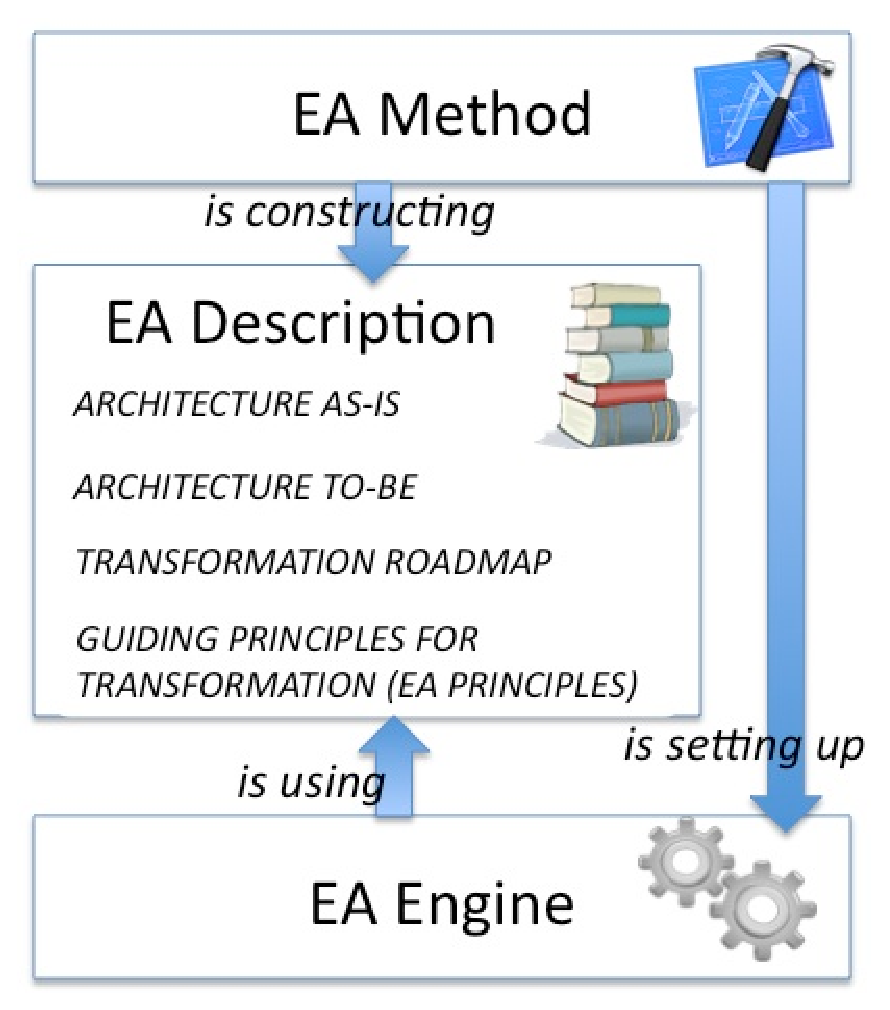
\includegraphics[scale=0.4]{EA}
\caption{Enterprise Architecture}
\label{fig:EA_general}
\end{figure}
In \cite{sachdeva1990}, organizational structure is defined as "... institutional arrangements and mechanisms for mobilizing human, physical, financial and information resources at all levels of the system..." Modern organizations are trending towards decentralization - where organizational units and individuals are being given an increasing amount of autonomy and control over an enterprise's direction and operations.

Decentralization transforms the role of company's authority and makes relationships inside and between different company's divisions much more complex. Planning and governance in different functional areas, including IT,  is not anymore ensured centrally. As a consequence, more efforts are required to prioritize initiatives, coordinate and communicate decisions, manage projects, and evaluate results. Moreover, the practices of management, coordination, communication and decision making are not the same as before: collaboration and information sharing gain extreme importance. This paper presents a taxonomy for categorizing these organizations on a spectrum ranging from centralized to decentralized. 

The de-facto EA methodologies rely on organizational properties such as centralized management, global company identity, etc.  that are getting obsolete with progressive decentralization.  Consequently, implementation of these methodologies in decentralized organization becomes difficult and inefficient and  the role of EA as a driver for IT transformations is getting compromised.

As an example, consider a public organization,  acquiring a software system with an objective of integrated facility management (room reservation etc.) (support of the services???) spanning across divisions that cost them thousands of euros. Divisions were not involved into decision making process and product evaluation (due to centralized strategic planning including IT planning) and eventually refused to shut down their local systems and switch to the global one ( due to decentralized IT management). As a consequence, strategic initiative for integration failed; divisions managed to protect their interests  (preserving local  systems  that  are  tailored for their needs) however got charged for the acquired system they never used (due to centralized budgeting). This example demonstrates a mismatch between the architecture principles (tendency towards integration), architecture engine (the process of prioritizing, evaluating and eventually deciding on the global system to adopt) and the organizational structure that inherits some centralized mechanisms while being strongly decentralized.

%In order for these EA frameworks to continue to be suitable for the modern enterprise, some changes need to be made to take into account these new enterprise structures. 


%They are taking for granted some organization and ICT properties (e.g. culture) that do not exist any more. As a result, the attempts to implement the EA methods or to follow the traditional principles meet the hostility in the organization (parts) and often fail.

Therefore, novel EA processes, principles and concepts are needed to both handle the ICT resources and to foster business/ICT co-evolution in decentralized environments.

This paper presents a literature review that supports our claim. The main contribution of this paper is a classification of organizational forms, used further to assess the prevalent EA methodologies and their obstacles in supporting decentralization, leading finally to a set of recommendations for decentralized-aware EA.

The reminder of this article is organized as follows: In Section II, we discuss the role of EA in organization and provides an overview of three EA methodologies: TOGAF, Zachman  and  FEA;  in  Section  III,  we  discuss  different forms of organizational structure and the trend towards decentralization. We conclude this section by highlighting the 4 (?) challenges related to decentralization in IT. In Section IV we analyze the EA methodologies presented in Section II focusing on their support to decentralization. We identify (5?? - a concrete number may sound good..) In Section V, we propose .......

% 
% Related EDOC aspects
%     Enterprise architecture frameworks 
%     (Collaborative development and cooperative engineering issues)
%     Enterprise interoperability, collaboration and its architecture
%     ([Cross-enterprise collaboration] in a world of cloud, social and big data)
% 
% 
% 
% 
% 
% 
% 
% 
% 
% 
% 
% 
% 
% 
% 
% 